\chapter{Experiential Learning of Networking Technologies: Understanding IP Routing}

\begin{center}
{\large\uppercase{$\text{Ram P. Rustagi}$}} 


\vskip -6pt

\end{center}

\vskip 2cm




\vfill




\newpage

\begin{multicols}{2}

In the previous article \cite{art2-key01}, we have studied assignment of IP address \cite{art2-key02} to a host, and its role in connecting to internet and communicating with other devices. We explored concept of a network number which is determined using IP address and subnet mask. When network number of two hosts is same, then these two hosts belongs to same network else these hosts belong to different networks. Hosts within the same network communicate directly with each other whereas hosts belonging to different network communicate using one or more intermediate routers. A router connects two networks, and its main job is to receive packets from one network and forward it to another network so as to enable the packet delivery towards its final destination. When two hosts are connected by many intermediate networks, communication between these two hosts require that each of the intermediate router in the path forward the packet on to the network which is closer to the destination and router in the last leg of this path will deliver the packet to destination host. In this article, we will explore this concept of packet forwarding and the mechanisms used to achieve this packet forwarding.

Consider the connectivity of two networks, say Network-1 and Network-2, as shown in Figure~\ref{chap2-fig01}. Each of these two networks consists of many connected systems (though as a representation only 2 are shown). Host $\textrm{H}_1$ and $\textrm{H}_2$ are part of Network-1, and Host $\textrm{H}_3$ and $\textrm{H}_4$ are part of Network-2. These two networks are connected via many intermediate routers, which we can consider as representing the internet. Host H1 and $\textrm{H}_2$ belongs to same network 10.x.x.0/24, and hence can communicate directly without requiring any intermediate router. Similarly, host $\textrm{H}_3$ communicates directly with $\textrm{H}_4$ as both belong to same network 10.y.y.0/24. However, when $\textrm{H}_1$ needs to communicate with $\textrm{H}_3$, the packets have to go through all the intermediate routers. When $\textrm{H}_1$ wants to send a packet to $\textrm{H}_3$, it will forward the packet to router $\textrm{R}_1$, which in turn will forward the packet to next router $\textrm{R}_2$, and so on, and finally Router $\textrm{R}_n$ will deliver the packet to host $\textrm{H}_3$. Thus, communication between two hosts involves routing of packets and primary focus of this article is to explore the mechanism used in forwarding these packets.

%~ \begin{figure}[H]
%~ \centering
%~ 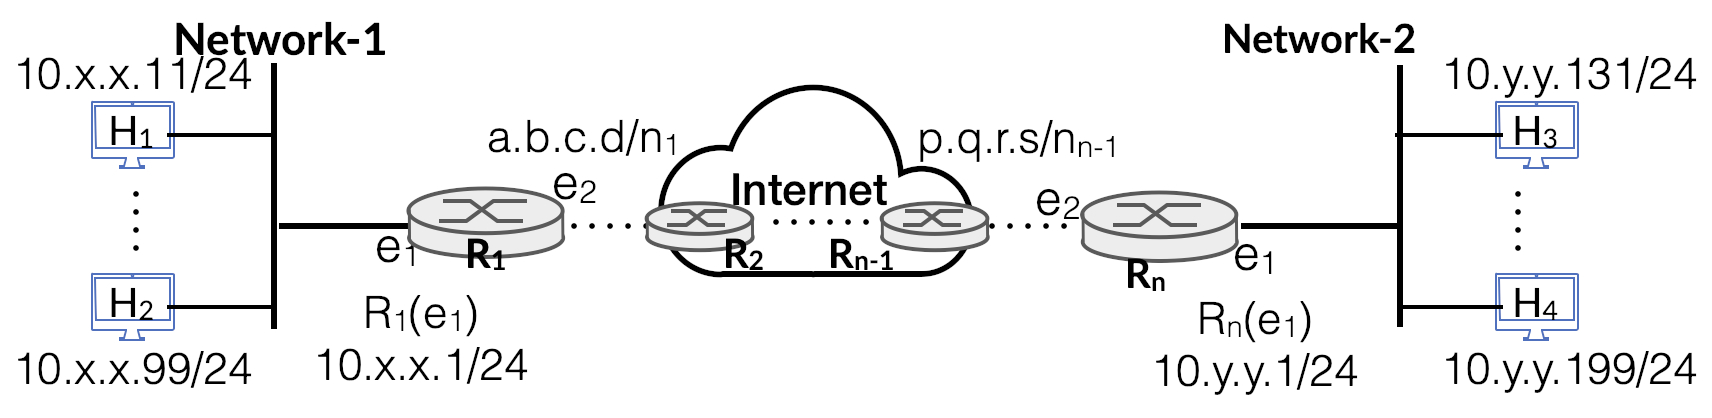
\includegraphics[scale=1.5]{src/Figures/chap2/chap2-fig01.jpg}
%~ \caption{Connectivity of two Networks, each network having many systems in it}\label{chap2-fig01}
%~ \end{figure}

Whenever, a host needs to send a packet to another hosts, it must know the IP address of destination host. For example, when we use browser to search at google.com, the machine where browser is running, finds the IP Address of gogole.com and then sets up TCP connection using IP address of google.com. When sending a packet, a host consults its routing table (also called as forwarding table) and determine the next hop in the path to destination host. Entries in the routing table plays a crucial role in how a host makes a packet forwarding decision. The routing decision using the routing table is always required irrespective of whether the destination host is in the same network or a different network.

\section{Routing Table Structure}\label{chap2-sec-1}

The main purpose of routing table is to help a host in determining the next hop where packet should be forwarded. The next hop could even be the next intermediate router or the final destination host itself. At its core, routing table has following four column fields, though in many implementations it may have some more information fields, such as cost metric etc., which we will not consider for our discussion.
\begin{itemize}
\item[i.] Destination Network.
\item[ii.] Subnet mask (for destination network).
\item[iii.] Network interface.
\item[iv.] Next hop or gateway router’s IP address.
\end{itemize}

A routing table would have number of row entries, with each row corresponding to a destination network. First two fields together identify a network, and are used to check if destination IP address of packet belongs to this network. If this entry matches, then packet is forwarded on the associated interface ($3^{rd}$ field) to the next hop ($4^{th}$ field). Next hop entry field is applicable when destination host is not connected to local network and identifies the IP address of next router in the forward path.  A typical set of entries for router $\rm{R}_1$ in Figure.~\ref{chap2-fig01} is given below in Table~\ref{chap2-table-1}, and routing entries for Host $\rm{H}_1$ is given in Table~\ref{chap2-table-2}.

\begin{table}[H]
\caption{Routing entries for $\rm{R}_{1}$}\label{chap2-table-1}
\begin{tabular}{|c|c|c|c|c|}
\hline
\textbf{S.N} & \textbf{Destination Network} & \textbf{Netmask} & \textbf{Interface} & \textbf{Next Hop}\\
\hline
1 & 10.x.x.0 &/24 & $\rm{e}_{1}$ & -\\
\hline
2 & a.b.c.d &/$\rm{n}_{1}$ & $\rm{e}_{2}$ & -\\
\hline
3 & \dots & \dots & \dots & \dots\\
\hline
4 & p.q.r.s & /$\rm{n}_{\rm{n}-1}$ & $\rm{e}_{2}$ & IP address of $\rm{R}_{2}$\\
\hline
5 & 10.y.y.0 & /24 & $\rm{e}_{2}$ & IP address of $\rm{R}_{2}$\\
\hline
6 & 0.0.0.0 & /0 & $\rm{e}_{2}$ & IP address of $\rm{R}_{2}$\\
\hline
\end{tabular}
\end{table}

\begin{table}[H]
\caption{Table 2: Routing entries for Host $\rm{H}_{1}$}\label{chap2-table-2}
\begin{tabular}{|c|c|c|c|c|}
\hline
\textbf{S.N.} & \textbf{Destination Network} & \textbf{Netmask} & \textbf{Interface} & \textbf{Next Hop}\\
\hline
1 & 10.x.x.0 & /24 & Ethernet & -\\
\hline
2 & 0.0.0.0 & /0 & Ethernet & 10.x.x.1\\
\hline
\end{tabular}
\end{table}

First two entries in Table~\ref{chap2-table-1} corresponds to two networks to which router $\rm{R}_{1}$ is directly connected and hence there is no next hop address. These will be followed by number of entries corresponding to network numbers that exist in the network. The entries in $4^{\rm th}$ and $5^{\rm th}$ row correspond to two networks connected with the router $\rm{R}_{n}$. Lastly, there is an entry corresponding to 0.0.0.0/0 which is also referred to as default route entry. Use of this default entry is explained ahead. For any host which is typically connected to a single network, there are generally two entries, as shown in Table~\ref{chap2-table-2} for host $\rm {H}_{1}$. One entry corresponds to local network and other entry corresponds to default network i.e. 0.0.0.0/0. These entries are sorted in the decreasing order of number of bits in netmask. For example, entry for netmask /27 will come before entries of netmask /26 or /25 etc.

\section{Using Routing Table to Forward Packets}\label{chap2-sec2}

When a host needs to send a packet to destination host or an intermediate router need to forward a received packet, then both the host and the router use a routing algorithm to determine how to send the packet to next hop or directly reachable destination host. An outline of such a routing algorithm is given in Table~\ref{chap2-table-3}. 

\begin{table}[H]
\caption{Routing Algorithm}\label{chap2-table-3}
\begin{tabular}{|cl|}
\hline
01: &  \#Algorithm For forwarding the packet\\
02: & Extract the destination address from the packet\\
03: & Repeat the following for each entry in routing table\\
04: & Apply the netmask ($2^{\rm nd}$ field) and compute network number\\
05: & Compare it with destination network ($1^{\rm st}$ field)\\
06: & If matche\\
07: & Forward packet to next-hop on listed interface ($3^{\rm rd}$ field)\\
08: & Exit // routing is over\\
09: & Else\\
10: & Continue to next entry\\
11: & When no match found (entry 0.0.0.0/0 not defined)\\
12: & Drop the packet\\
13: & Inform the sender (ICMP error message)\\
\hline
\end{tabular}
\end{table}

Consider the network given in Figure~\ref{chap2-fig01}, and that host ${\rm H}_{1}$ (belonging to Network-1) needs to send a packet to host ${\rm H}_{3}$ (belonging to Network-3). Thus the source and destination addresses of this packet would correspond to 10.x.x.11 and 10.y.y.131. Routing algorithm makes uses of only the destination address and does not consider the source address, and works as follows. Routing table of host ${\rm H}_{1}$ (Table~\ref{chap2-table-2}) has just two entries. Using the destination address 10.y.y.131 (as extracted from the IP packet in line 02 of), the lines 03 to 10 of routing algorithm will be applied to this destination address. Applying the netmask /24 of first entry in the routing table (Table~\ref{chap2-table-2}) to destination address 10.y.y.131 (line 04), network number is computed as 10.y.y.0. For a detailed discussion on computation of network number, reader can review the article by as given in \cite{art2-key01}. Comparison (line 05) of computed network number with destination network 10.x.x.0 for first entry fails and hence routing process repeats as per line 09-10 for the next entry. For the $2^{\rm nd}$ entry (Table~\ref{chap2-table-2}), netmask is /0, and applying this netmask to 10.y.y.131 gives the network number as 0.0.0.0. This computed network number matches with destination network in $2^{\rm nd}$ entry of routing table of ${\rm H}_{1}$, and thus packet is forwarded to router ${\rm R}_{1}$ on Ethernet interface of host ${\rm H}_{1}$. Applying netmask /0 with any IP address will always compute the network number as 0.0.0.0 and thus it will always match the destination network and therefore this is called the default route entry i.e. when no other routing entry matches, this entry will always match. The default route entry in a routing table always appears as the last entry.

\section{Delivering Packet to Next Hop and ARP Protocol}\label{chap2-sec3}

When host ${\rm H}_{1}$ is sending the packet to host ${\rm H}_{3}$, it only contains source IP address (${\rm H}_{1}$) and destination IP address (${\rm H}_{3}$). The packet does not have IP Address of either router ${\rm R}_{1-}$ or any of the intermediate router(s). So, it is important to understand the mechanism used in delivering this packet to router ${\rm R}_{1}$ (next hop address). Any system is connected to a network via its link layer adaptor e.g. ethernet interface. Each link layer adaptor has its link layer address, also known as MAC (Medium Access Control) Address for ethernet adaptors. MAC address is a popular term and thus in general, any link layer address is called as MAC address. The MAC address consists of 6 bytes and generally written in hexadecimal notation. Windows system use dash as separator of two bytes, and therefore, MAC address in a windows system will be shown as xx-xx-xx-xx-xx-xx. In Linux, colon(:) is used as the separator and thus MAC address is shown as xx:xx:xx:xx:xx:xx.  An interesting property of MAC address is that it is unique across the world i.e. no two adaptors can have same MAC Address. The MAC address is assigned by link adaptor manufacturer and entire MAC Address space is managed by IEEE (Institute of Electrical and Electronic Engineers). Thus, whenever anyone wants to manufacture the link layer adaptors, they need to get a block of addresses (corresponding to first 3 bytes of MAC address) from IEEE and assign the remaining 3 bytes uniquely to each of the adaptor that company will manufacture. Thus, MAC address is not configurable by a user and is fixed with the adaptor whereas IP address is user configurable and assigned by a network administrator.

Whenever a machine sends a packet, the packet goes out from the link layer adaptor, which inserts its MAC address as the source MAC address in the transmitted frame. The sender also needs to correctly fill the destination MAC Address field in the transmitted frame, which is required for receiving host to receive and process it.  When link layer adaptor of receiving host receives a frame, it compares the received destination MAC address in the frame with its own MAC Address. Only when two addresses match, the adaptor receives the frame, extracts the network layer packet and passes it on to host for further processing by upper layer network stack. If the MAC address match fails, then adaptor simply discards the frame and network layer will not even see this packet. A link layer adaptor also receives and processes all those frames which have destination MAC address set as broadcast MAC address (all bits in the MAC address field are set to 1) and written as FF:FF:FF:FF:FF:FF.

Thus, for host ${\rm H}_{1}$ to forward the packet to router ${\rm R}_{1}$ (Figure~\ref{chap2-fig01}), it must fill the MAC address of the network interface ${\rm e}_{1}$ of router in the transmitted frame. From the routing table, it only knows the IP address of router ${\rm R}_{1}$. The MAC address of ${\rm R}_{1}$(${\rm e}_{1}$) interface, let say it is ${\rm MAC}_{\rm R1(e1)}$, is known only to ${\rm R}_{1}$. Unless the sender host fills this MAC address in the frame being sent, ${\rm R}_{1}$ will never receive this packet. Thus, we need a protocol that enables a sender host to obtain the MAC address corresponding to IP Address of receiver host. This functionality is provided by Address Resolution Protocol (ARP) \cite{chap2-key03}. ARP protocol enables the sender host to find out the MAC address of next hop (immediate recipient of packet) given its IP Address. The protocol works as follows. Sender host broadcasts an ARP Request message to all machines in the local network by setting the destination MAC address as broadcast address i.e. FF:FF:FF:FF:FF:FF. This ARP request message is received by all the machines in the local network as its destination MAC address is broadcast address. Link layer adaptor of each host receives this frame, extracts the network packet from it, and passes this request message to ARP module (network layer) for further processing. ARP module of each hosts compares the IP address in the received ARP Request message with its own IP address.  If the match fails, then ARP module simply discards the message. This match will fail for all systems except one (whose IP Address matches). For example, ${\rm H}_{1}$ will send ARP Request asking for MAC address corresponding to IP Address 10.x.x.1 (${\rm e}_{1}$ interface of ${\rm R}_{1}$). The ARP module of router will find the match successful since ARP Request is for its own IP Address and all other hosts in Network-1 will discard this ARP request message. The router ${\rm R}_{1}$ then responds with ARP Reply message providing MAC Address of its ${\rm R}_{1}$(${\rm e}_{1}$) interface. ${\rm R}_{1}$ already knows the MAC address of ${\rm H}_{1}$ since this was the source MAC address when ARP request message was received and thus it does not need to make another ARP Request. When ${\rm H}_{1}$ receives the ARP Reply, it makes a note of the MAC address of ${\rm R}_{1}$(${\rm e}_{1}$) and stores it in its ARP table.

Now for the original data packet that ${\rm H}_{1}$ wants to send to ${\rm H}_{3}$, the link layer frame sent by ${\rm H}_{1}$ will have source MAC of ${\rm H}_{1}$ and destination MAC corresponding to ${\rm R}_{1}$(${\rm e}_{1}$) interface, source IP as 10.x.x.11 (${\rm H}_{1}$) and destination IP as 10.y.y.131 (${\rm H}_{3}$). When this packet is transmitted by ${\rm H}_{1}$, link layer adaptor of ${\rm R}_{1}$ will receive this frame and pass it to higher layer of router which will process it further. The router ${\rm R}_{1}$ will apply its routing algorithm () to determine the next hop. Routing algorithm will evaluate entries from the routing table (Table\ref{chap2-table-1}) one at a time till it finds a match for the destination IP of 10.y.y.131. The first entry will compute network number as   10.y.y.0 which does not match destination network ($1^{\rm st}$ field) 10.x.x.0 and thus routing algorithm evaluates $2^{\rm nd}$ entry. Again, this will not match and process goes on for remaining entries. The match will occur for $5^{\rm th}$ entry where computed network number is 10.y.y.0 as well as destination network ($1^{\rm st}$ field) for $5^{\rm th}$ entry is also same. Thus, router will forward the packet to next hop router ($4^{\rm th}$ field) ${\rm R}_{2}$. Routing algorithm only provides the IP address of next hop router and not the MAC address. Router ${\rm R}_{1}$ will follow the same process as described earlier to find the MAC address of ${\rm R}_{2}$’s network interface. ${\rm R}_{1}$ will send ARP request for ${\rm R}_{2}$, ${\rm R}_{2}$ will respond with ARP Reply and then ${\rm R}_{1}$ will forward the packet with source IP as 10.x.x.11 and destination IP as 10.y.y.131 to ${\rm R}_{2}$. This link layer frame will have source MAC corresponding ${\rm R}_{1}$(${\rm e}_{2}$), and destination MAC corresponding to ${\rm R}_{2}$ (network interface). When ${\rm R}_{2}$ receives this packet, it will follow the same process of finding the MAC address of next hop router, forward the data packet with source IP as 10.x.x.11 and destination IP as 10.y.y.132 and forward it to next hop router. This process will be followed at each intermediate router till last router ${\rm R}_{\rm n}$ receives this packet and delivers this packet to ${\rm H}_{3}$. Thus, in each hop, source IP and destination IP remains the same, but source MAC and destination MAC will change on per hop (link layer connectivity) basis.

The set of steps for experiential exercise to understand the packet delivery within the same network is given in Exercise~\ref{chap2-exe1}.

\section{Constructing Routing Table}\label{chap2-sec4}

Internet consists of many networks which are connected by a number of routers. A router needs to build its routing table so as to be able to forward the packet correctly in the right direction towards the destination. Building of routing table can be done either manually (e.g. network admin configuring the routing table of each involved router) or dynamically by routers themselves. When number of networks are large, it is infeasible to build the routing table manually. However, to understand its construction and get an experiential exposure, we will first explore the process of building a routing table manually and later on briefly dwell upon building these dynamically. To build these tables manually, consider a simple network consisting of three hosts ${\rm H}_{1}$, ${\rm H}_{2}$ and ${\rm H}_{3}$ (as shown in Figure~\ref{chap2-fig02}), where each host is associated with multiple networks. This simple network setup is sufficient to lay the foundation of routing table construction.

%~ \begin{figure}[H]
%~ \centering
%~ 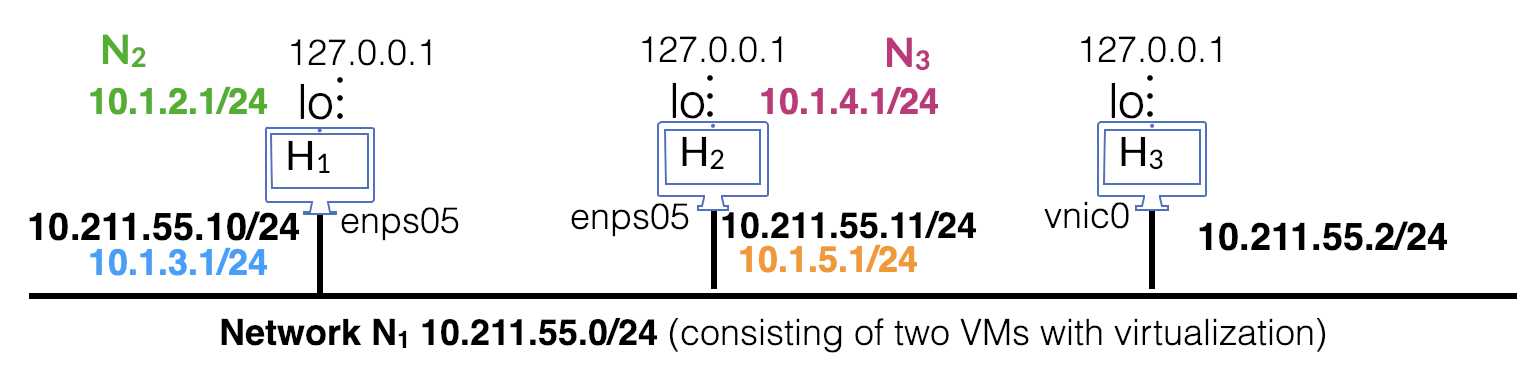
\includegraphics[scale=1.5]{src/Figures/chap2/chap2-fig02.jpg}
%~ \caption{Multi network connectivity using VMs}\label{chap2-fig02}
%~ \end{figure}

From implementation perspective of this network, a typical reader of this article would have access to a single laptop, and thus we will make use of virtual machines to setup such a network. This requires installing some virtualization software, such as VirtualBox\cite{art2-key07}, VMWare\cite{art2-key09}, Parallels\cite{art2-key08} (only for Mac) etc., on the host system (i.e. laptop running Windows, or Macbook etc.). The above depicted network is created using 2 Virtual Machines running Ubuntu\footnote{Any other version of Ubuntu would work equally well.} 16.4LTS (${\rm H}_{1}$) and 18.4LTS (${\rm H}_{2}$) along with the host OS (${\rm H}_{3}$). Author of this article is using Macbook (host ${\rm H}_{3}$) as the host OS and has created the Ubuntu VMs using Parallels\cite{art2-key08} virtualization software. The network 10.211.55.0/24 is created by virtualization software and all VMs attach to this network. Two Ubuntu VMs (${\rm H}_{1}$ and ${\rm H}_{2}$) get their respective network addresses as 10.211.55.10/24 and 10.211.55.11/24 and host system is assigned the IP address 10.211.55.2/24. As all 3 systems belong to same network, these can communicate with each other directly without requiring any connecting router.


Understanding of routing and building a routing table requires us to work with more than one network. Though at the time of VM invocation, they belong to only one network, we will create 4 more networks, and assign two networks to each of Ubuntu VM using its ethernet interface en0s5 as well as loopback lo interface. We will make use of the phenomenon of assigning a number of network addresses (even belonging to different networks) to a network interface.  Table~\ref{chap2-table-4} and Table~\ref{chap2-table-5} respectively provide Linux commands to assign multiple IP addresses to interfaces of hosts ${\rm H}_{1}$ and ${\rm H}_{2}$. Line 01 (Table~\ref{chap2-table-4}) shows the existing IP addresses belong to loopback and ethernet interfaces of host ${\rm H}_{1}$.  Lines 02 and 03 assign the new network addresses respectively to loopback and ethernet interfaces. These new addresses are in addition to existing addresses and same is shown in output of command at line 04. Similarly, lines 01-04 (Table~\ref{chap2-table-5}) shows the assignment of new network addresses to host ${\rm H}_{2}$. The ethernet interface name would vary depending upon VM Ubuntu installation, and thus reader should appropriately replace it in the network setup being created for experiential learning as described in.
\begin{table}[H]
\caption{Assigning Multiple IP Addresses to host ${\rm H}_{1}$}
\begin{tabular}{|l@{\;}l|}
\hline
\# & Assigning addresses to host ${\rm H}_{1}$\\
\# & Addresses on power up of ${\rm H}_{1}$\\
01:& ${\rm H}_{1}$> ip -4 addr show\\
1: & lo: <LOOPBACK,UP,LOWER\_UP> mtu 65536 $\ldots$\\
   & \quad inet 127.0.0.1/8 scope host lo $\ldots$\\
2: & enp0s5: <BROADCAST,MULTICAST,UP,LOWER\_UP> mtu 1500 $\ldots$\\
   & \quad inet 10.211.55.10/24 brd 10.211.55.255 scope global dynamic enp0s5 $\ldots$\\
   \hline
\# & Assigning new network addresses to enp0s5 and lo interface of ${\rm H}_{1}$\\
02:& ${\rm H}_{1}$> sudo ip addr add 10.1.2.1/24 dev lo\\
03:& ${\rm H}_{1}$> sudo ip addr add 10.1.3.1/24 dev enp0s5\\
\hline
\# & Verification of new addresses on ${\rm H}_{1}$\\
04:& ${\rm H}_{1}$> ip -4 addr show\\
1: & lo: <LOOPBACK,UP,LOWER\_UP> mtu 65536 $\ldots$\\
   &\quad inet 127.0.0.1/8 scope host lo $\ldots$\\
   & \quad inet 10.1.2.1/24 scope global lo $\ldots$\\
2: & enp0s5: <BROADCAST,MULTICAST,UP,LOWER\_UP> mtu 1500 $\ldots$\\
   & \quad inet 10.211.55.10/24 brd 10.211.55.255 scope global dynamic enp0s5 $\ldots$\\
   &\quad inet 10.1.3.1/24 scope global enp0s5 $\ldots$\\
   \hline   
\end{tabular}
\end{table}

\begin{table}[H]
\caption{Assigning Multiple IP Addresses to Host ${\rm H}_{2}$}\label{chap2-table-5}
\begin{tabular}{|l@{\;}l|}
\hline
\# & Assigning addresses to host ${\rm H}_{1}$\\
\# & Addresses on power up of ${\rm H}_{1}$\\
01:& ${\rm H}_{2}$ > ip -4 addr\\
1: & lo: <LOOPBACK,UP,LOWER\_UP> mtu 65536 $\ldots$\\
    &\quad inet 127.0.0.1/8 scope host lo $\ldots$\\
2: & enp0s5: <BROADCAST,MULTICAST,UP,LOWER\_UP> mtu 1500 $\ldots$\\
   & \quad inet 10.211.55.11/24 brd 10.211.55.255 scope global $\ldots$ enp0s5 $\ldots$\\
    \hline
\# & Assigning new addresses to enp0s5 and lo interface of ${\rm H}_{2}$\\
02: & ${\rm H}_{2}$ > sudo ip addr add 10.1.4.1/24 dev lo\\
03: & ${\rm H}_{2}$ > sudo ip addr add 10.1.5.1/24 dev enp0s5\\
\hline
\# & Verification of new addresses on ${\rm H}_{2}$\\
04:& ${\rm H}_{2}$ > ip -4 addr\\
1:& lo: <LOOPBACK,UP,LOWER\_UP> mtu 65536 $\ldots$\\
   & \quad inet 127.0.0.1/8 scope host lo $\dots$\\
   &  \quad inet 10.1.4.1/24 scope global lo $\ldots$\\
  \hline 
2:& enp0s5: <BROADCAST,MULTICAST,UP,LOWER\_UP> mtu 1500 $\ldots$\\
   & \quad inet 10.211.55.11/24 brd 10.211.55.255 scope global $\ldots$ enp0s5 $\ldots$\\
   & \quad inet 10.1.5.1/24 scope global enp0s5 $\ldots$\\
   \hline
\end{tabular}
\end{table}

With the creation of 4 new networks, host ${\rm H}_{1}$ does not know the route to reach the network 10.1.4.0/24 and 10.1.5.0/24. Similarly, host ${\rm H}_{2}$ does not know how to reach the networks 10.1.2.0/24 and 10.1.3.0/24. Reachability to these networks requires creation of routing entries in the routing tables of ${\rm H}_{1}$ and ${\rm H}_{2}$ respectively. Host ${\rm H}_{1}$ (IP address 10.211.55.10) can reach both 10.211.55.11(${\rm H}_{2}$) and 10.211.55.2(${\rm H}_{3}$) as all three addresses belongs to same network with network number 10.211.55.0/24. Similarly, host ${\rm H}_{2}$ (10.211.55.11) can reach both 10.211.55.10(${\rm H}_{1}$) and 10.211.55.2(${\rm H}_{3}$). The networks 10.1.4.0/24 and 10.1.5.0/24 are reachable via 10.211.55.11(${\rm H}_{2}$) and thus ${\rm H}_{2}$ can act as gateway for these two networks. Similarly, networks 10.1.2.0/24 and 10.1.3.0/24 are reachable via 10.211.55.10 (${\rm H}_{1}$), and thus ${\rm H}_{1}$ can act as gateway for these two networks. 

Using this reachability knowledge of these new networks, routing table entries for these networks on ${\rm H}_{1}$ and ${\rm H}_{2}$ are created using each other as the gateway. The commands to create the routing entries are shown in Table~\ref{chap2-table-6}. The command “ip route add” (lines 02-03) has basically four parameters corresponding to four fields of the routing table (Table~\ref{chap2-table-1}). As ${\rm H}_{1}$ and ${\rm H}_{2}$ are hosts (end systems) and are connected to multiple networks, these systems are known as multi-homed hosts, as a host either consumes (receives) or generates (sends) a packet. To enable routing functionality in a host so that it can forward packets across the connected networks, it needs to be configured as a router i.e. forward packets across interfaces/networks. The commands in Table~\ref{chap2-table-6} at line 01 and 05 enable routing functionality in these two hosts. Line 02 (Table~\ref{chap2-table-6}) adds the routing entry for network 10.1.4.0/24, next hop gateway as 10.211.55.11 (${\rm H}_{2}$) and packet has to be sent out on interface enp0s5. Similarly, command at line 03 adds the routing entry in ${\rm H}_{1}$ for $2^{\rm nd}$ network 10.1.5.0/24. Similarly, lines 06-07 demonstrate creation of routing entries in host ${\rm H}_{2}$.

\begin{table}[H]
\caption{Creating Routing table}\label{chap2-table-6}
\begin{tabular}{|l@{\;}l|}
\hline
\# & Creating routing table at ${\rm H}_{1}$\\
01:& ${\rm H}_{1}$> sysctl -w net.ipv4.ip\_forward=1\\
02:& ${\rm H}_{1}$> sudo ip route add 10.1.4.0/24 via 10.211.55.11 dev enp0s5\\
03:& ${\rm H}_{1}$> sudo ip route add 10.1.5.0/24 via 10.211.55.11 dev enp0s5\\
04:& ${\rm H}_{1}$> ip -4 route show\\
   &\quad default via 10.211.55.1 dev enp0s5  proto static metric 100 \\
   &\quad 10.1.3.0/24 dev enp0s5  proto kernel  scope link src 10.1.1.1 \\
   &\quad 10.1.4.0/24 via 10.211.55.11 dev enp0s5 \\
   &\quad 10.1.5.0/24 via 10.211.55.11 dev enp0s5 \\
   &\quad 10.211.55.0/24 dev enp0s5 proto kernel scope link src 10.211.55.10\\
\hline
\# & Creating routing table at ${\rm H}_{2}$\\
05:& ${\rm H}_{2}$> sysctl -w net.ipv4.ip\_forward=1\\
06:& ${\rm H}_{2}$> sudo ip route add 10.1.2.0/24 via 10.211.55.10 dev enp0s5\\
07:& ${\rm H}_{2}$> sudo ip route add 10.1.3.0/24 via 10.211.55.10 dev enp0s5\\
08:& ${\rm H}_{2}$> ip -4 route show\\
   &\quad default via 10.211.55.1 dev enp0s5 proto dhcp metric 100\\ 
   &\quad 10.1.2.0/24 via 10.211.55.10 dev enp0s5\\ 
   &\quad 10.1.3.0/24 via 10.211.55.10 dev enp0s5\\
   &\quad 10.1.5.0/24 dev enp0s5 proto kernel scope link src 10.2.1.1 \\
   &\quad 10.211.55.0/24 dev enp0s5 proto kernel scope link src 10.211.55.11\\
\hline
\end{tabular}
\end{table}
\end{multicols}
